% Chapter Template

\chapter{Soluciones presentadas} % Main chapter title
\label{cap:soluciones} % Change X to a consecutive number; for referencing this chapter elsewhere, use \ref{ChapterX}

\section{Metodología}
\label{sec:metodology}

La puntuación final de la competición será calculada mediante una función de pérdida logarítmica, como vimos en el apartado \ref{sec:envio-y-eval}. Al no tener las categorías del conjunto de datos de test debemos delegar el cálculo de la puntuación en Kaggle, que permite enviar hasta cinco predicciones al día. Esto es un obstáculo para hacer pequeñas pruebas e iterar rápido sobre los resultados. Por otra parte, el segundo conjunto de test tiene más de 13000 imágenes, que no son rápidas de cargar en memoria ni de pasar por el modelo que se genere. En determinados casos la evaluación del segundo conjunto de test ha tardado más de 6 horas.

La solución a este problema se ha resuelto usando un subconjunto del conjunto de entrenamiento dedicado solo a la evaluación de modelos. Por otra parte, para el entrenamiento es necesario usar un subconjunto de validación, por lo tanto es necesario dividir el conjunto de entrenamiento original en tres subconjuntos: entrenamiento, validación y test.

La partición se ha realidado dejando un \textbf{60\%} de los datos al conjunto de entrenamiento, un \textbf{20\%} al conjunto de validación y un \textbf{20\%} al conjunto de test.


\subsection{Partición de conjuntos de datos}
La partición del conjunto de datos es una operación delicada. Ya vimos que uno de los problemas del dataset era que la cantidad de imágenes para cada clase era muy variada, teniendo algunas clases un número muy bajo de ejemplos. Si sacamos el 40\% de las imágenes del dataset, podemos estar vaciando una o varias categorías de ejemplos de entrenamiento, haciendo inútil cualquier clasificación de esas clases.

La solución por la que se ha optado es generar un subconjunto del 20\% usando el 20\% de los ejemplos de cada clase, evitando así vaciar alguna de las clases.

\subsection{Evaluación del modelo}

Para una búsqueda más óptima de parámetros y configuraciones el modelo se evaluará contra el grupo de test generado. Una vez se encuentren determinados modelos especialmente interesantes por tener una puntuación máxima local entre aquellos a los que se compara habrá que enviarlo a Kaggle para su evaluación completa.

Enviar el modelo a Kaggle se puede hacer sobre una partición más grande del conjunto de entrenamiento, ya que no es necesario usar un conjunto de test para evaluar, solo uno de validación. Esto permite entrenar el modelo sobre el 80\% de los datos consiguiendo, por lo general, resultados más precisos.

\subsection{Software}

Todos los modelos de redes convolucionales que se van a entrenar en este proyecto han sido entrenados usando Keras
\section{Idea}
A la hora de afrontar este problema de clasificación de peces es lógico
seguir una estrategia separada en dos pasos: primero buscar si
existe un pez en la foto y luego intentar clasificarlo en una de las 
categorías existentes. 

Para encontrar un pez en la foto es necesario encontrar una serie de
características que puedan ser identificadas con algún pez. La idea de 
la solución parte de esta base. A la hora de clasificar una imagen
primero es necesario encontrar el contenido relevante para ser usado
en la clasificación.

Como ya se comentó al hablar de las redes convolucionales (capítulo \ref{sec:conv-net-arch}),
las arquitecturas encontradas en problemas similares \parencite{krizhevsky2012imagenet}
permiten separar con claridad estas dos etapas mediante el uso de redes convolucionales (CONV) y capas densas (FC).

\section{Arquitectura}

La arquitectura general usada, que luego sufrirá pequeños cambios, es la descrita en la figura~\ref{general-architecture} (Krizhevsky et al.)

\begin{figure}
  \caption{Arquitectura de la red en dos partes}
\label{general-architecture}
  \makebox[\textwidth]{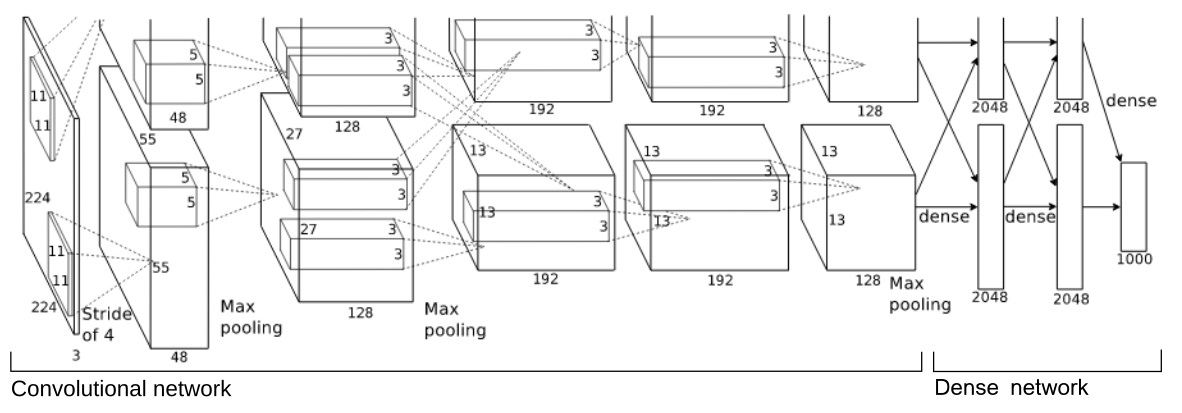
\includegraphics[width=\linewidth]{imagenet-arch}}
\end{figure}

Esta arquitectura usa en su primera parte una red convolucional preentrenada sobre un conjunto de imágenes mucho más generalista, en este caso Imagenet. Al usar una red convolucional preentrenada sobre fotografías tendrá muchas más capacidad para distinguir características de diferentes objetos, además que existen varias categorías de peces en Imagenet, por lo que sabrá diferenciar este tipo de fotografías.


\subsection{Red convolucional}

Como explicamos en el capítulo~\ref{sec:conv-net}, cuando un modelo convolucional recibe una imagen va a devolver $N$ matrices bidimensionales representando el resultado de las aplicación de los $N$ conjuntos de filtros a la imagen inicial. Al ser $N$ matrices bidimensionales también puede considerarse una matriz tridimensional.

Intuitivamente, y haciendo una simplificación, podemos pensar que cada uno de estos filtros representa un mapa de calor de la aparición en la imagen de diferentes características. Por ejemplo, ¿cúanto se parece cada parte de esta imagen a la piel de un pez?.

Hay que tener en cuenta que este modelo convolucional no ha sido entrenado con el conjunto de entrenamiento, si no con el conjunto de entrenamiento de Imagenet. Para lo único que vamos a usar esta red convolucional es para transformar estas imágenes a 

\subsection{Modelo preentrenado}

La arquitectura del artículo original \parencite{krizhevsky2012imagenet} usa capas convolucionales donde alterna filtros de $11\times11$, $5\times5$, y $3\times3$, el cual parece una buena elección para usar como modelo convolucional preentrenado. Sin embargo la aplicación de este trabajo es una competición internacional donde se usarán soluciones \textit{state of the art}. El modelo de la figura \ref{general-architecture} representa el ganador de la edición 2012 de la competición ILSVRC. Un buen punto de partida puede ser mirar los modelos ganadores de años posteriores.

El modelo principal a usar es VGG, desarrollado por el \textit{Visual Geometry Group}, de la Universidad de Oxford. Es un modelo especialmente interesante por su simplicidad, aparte de obtener una de las mejores puntuaciones en ILSVRC 2014.

\section{VGG16}

Una de las principales características de VGG es la idea de que los filtros convolucionales mayores de $3\times3$, como por ejemplo los de $5\times5$ u $11\times11$ pueden ser representados por combinaciones de filtros $3\times3$.

De las configuraciones descritas en \parencite{simonyan} hay una que sobresale por su eficiencia, llamada VGG16. Usando un total de trece capas CONV con filtros de $3\times3$, cinco capas POOL y tres capas FC (de 4096, 4096 y 1000 salidas), seguida de una función \textit{softmax} (figura \ref{vgg16-arch}), es capaz de mejorar la eficacia del modelo de Krizhevsky. El nombre de esta configuración es VGG16 ya que es la cantidad de capas CONV y FC que posee.

Estamos usando la configuración VGG16 de todas las descritas en su definición original ya que, junto con VGG19, consigue los mejores resultados.

\begin{figure}
  \caption{Arquitectura de VGG}
\label{vgg16-arch}
  \makebox[\textwidth]{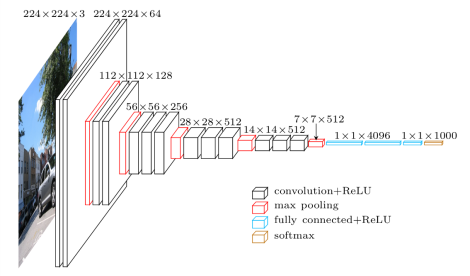
\includegraphics[width=.7\linewidth]{vgg16-arch}}
\end{figure}

\subsection{\textit{Fine-tuning}}

Si observamos la última capa del modelo VGG16, vemos que la salida tiene 1000 elementos. Tiene esta forma ya que ILSVRC consistía en clasificar una imagen entre mil categorías diferentes. Si el problema a resolver consiste en clasificar entre ocho categorías, es lógico modificar esta última capa para que tenga solo ocho salidas.

Al modificar la estructura de la última capa estamos destruyendo pesos y haciendo que muchos de los que ya existían carezcan de sentido. El hecho de que VGG tenga esta separación lógica entre la red convolucional y la red densa (las tres capas FC) hace que se pueda separar el modelo en dos modelos diferentes: uno convolucional, que no habrá cambiado con la adaptación a las ocho categorías, y otro denso, que tendrá que ser reentrenado de nuevo.

Al partir una red en dos partes diferentes hay que tener en cuenta que la segunda parte, la red densa, no recibe como entrada las imágenes, si no la salida de la red convolucional, con todas las transformaciones que esta produce. Es necesario entonces aplicar la red convolucional a todo el conjunto de datos para crear un nuevo conjunto de datos con el que reentrenar la red densa.

Esta técnica de ajustar los paŕametros de un modelo ya conocido para adaptarlo con nuevo conjunto de datos se conoce como \textit{fine-tuning}.

Usando el conjunto de datos definido en el capítulo \ref{sec:metodology}, con la separación 60\%, 20\% y 20\% para los conjuntos de entrenamiento, validación y test se ha entrenado la red densa.

Primero es necesaria la transformación del conjunto en las features producidas por la red convolucional.

\begin{python}
# Carga del modelo VGG16
from vgg16 import Vgg16
model = Vgg16()

# Diferencia entre red convolucional y densa
import utils
conv_model, dense_model = utils.split_at(model, MaxPooling2D)

# Cargamos los diferentes conjuntos de datos
train, trail_labels = get_data(path + 'train')
valid, valid_labels = get_data(path + 'valid')
test, test_labels = get_data(path + 'test')

# Convertir dataset a features mediante la red convolucional 
train_feat = conv_model.predict(train)
valid_feat = conv_model.predict(valid)
test_feat = conv_model.predict(test)
\end{python}

Este código no es completamente válido, ya que se han tomado algunas libertades para mejorar la comprensión y lectura del mismo. Define una estructura general a seguir para este problema (carga de datos, transformación, \textit{fine-tuning} y evaluación). Para una mayor comprensión el la mayor parte de las librerías usadas así como las utilidades están descritas en el Apéndice 1 (cuando lo pase a LaTex)

Una vez cargadas las librerías necesarias (Vgg16 es una clase abstracta que importa las bibliotecas necesarias de Keras), ambos modelos y transformado el dataset mediante la red convolucional se puede pasar a reentrenar la última parte de la red. Primero hay que cambiar el final de la red para conseguir que tenga ocho salidas y luego entrenar.


\begin{python}

# Cambiar el final de la red densa de 1000 outputs a 8
dense_model.pop()  # Elimina la última capa
dense_model.add(
    Dense(8, activation='softmax')  # Introducir una nueva
)

# Compilar el modelo
dense_model.compile(
    SGD(lr=0.01),
    loss='categorical_crossentropy',
    metrics=['accuracy'],  # Muestra la precision del modelo
)

# Entrenar la red
dense_model.fit(
    train_feat,
    train_labels,
    batch_size=64,  # Numero de imagenes a entrenar al mismo tiempo
    nb_epoch=7,     # Numero de iteraciones del entrenamiento
    validation_data=(valid_feat, valid_labels),
)

# Evaluar el modelo sobre el conjunto de test
dense_model.evaluate(test_feat, test_labels)
# Log loss, accurtcy
>>> [2.38985158622892523, 0.66099843993759748]
\end{python}

La puntuación total de kaggle para este conjunto de test sería $2.389$. Esto es sobre un conjunto de test muy pequeño, solo el 20\% del conjunto de entrenamiento. Como se ya ha dicho anteriormente habría que mandar las predicciones del conjunto de test final a kaggle para verificar la puntuación del modelo, pero por problemas de restricciones esta es la forma de medir los modelos generados.

El segundo número que devuelve la función $evaluate$ es la precisón ($accuracy$) del modelo. Al ser el modelo un modelo de clasificación, el mandar $"accuracy"$ como parámetro a la hora de compilar el modelo hace que eliga como métrica la precisión por categorías. Esto va a devolver el porcentaje de veces que la clase con la probabilidad máxima se corresponde con la clase etiquetada en el dataset. En este caso el modelo ha adivinado correctamente el 66\% de las imágenes, un número muy aceptable teniendo en cuenta que solo se ha tocado la capa final de un modelo ajeno.

\section{Modelo completamente conectado}

La idea original que se comentaba al principio consistía en separar el problema en el modelo convolucional y el modelo de clasificación. Es en el segundo donde se puede conseguir toda la flexibilidad. 

El modelo original de VGG usa dos capas $densas$ de 4096 neuronas para clasificar entre mil clases diferentes. Ya que este problema tiene solo ocho clases diferentes probablemente no sea necesario usar capas tan grandes, por lo que se procede a probar la misma estructura original pero con capas cuatro veces más pequeñas que las originales.

La estructura, por lo tanto, quedaría de la misma manera pero usando dos capas densas de 512 neuronas cada una y una capa densa final de 8. Para no tener que estar modificando el modelo original cada vez que haga falta es mucho más sencillo crear un modelo nuevo con $Keras$ y añadir todas las capas necesarias.

\begin{python}
def build_dense_layers():
    return [
        Flatten(),
        Dense(512, activation='relu'),
        Dense(512, activation='relu'),
        Dense(8, activation='softmax')
    ]

dense_model = keras.models.Sequential(build_class_layers())
\end{python}

Un paso importante a la hora de construir el modelo personalizado es tener en cuenta que las salidas de las redes convolucionales poseen tres dimensiones ($ancho \times alto \times filtros$), mientras que la redes neuronales densas poseen solo una dimensión. Es necesario convertir la salida de estas capas a una entrada permitida. Keras ya ofrece esta posibilidad usando una capa abstracta llamada Flatten.

\begin{python}
# Entrenar la red
dense_model.compile(...)
dense_model.fit(...)
# Evaluar el modelo sobre el conjunto de test
dense_model.evaluate(test_feat, test_labels)
>>> [1.27161316430079874, 0.73067862714508579]
\end{python}

Los resultados obtenidos son ligeramente mejores que los anteriores, sin embargo no es aquí donde está toda la mejora. El entrenamiento de este modelo ha sido un 80\% más rápido que el anterior (19.5 segundos el primero, 3.9 segundos el último). Esto no solo ha permitido entrenar la red durante más tiempo, si no que en el futuro hará posible entrenar sobre mayores cantidades de datos sin sacrificar velocidad.

\subsection{Mejorar el modelo}

La salida de Keras al entrenar el modelo ofrece información de lo que está sucediendo. Este es un ejemplo de la salida del entrenamiento del modelo anterior.

\begin{python}
Epoch 5/7
loss: 1.406 - acc: 0.621 - val_loss: 2.0197 - val_acc: 1.861
Epoch 6/7
loss: 0.992 - acc: 0.674 - val_loss: 1.4356 - val_acc: 1.001
Epoch 7/7
loss: 0.872 - acc: 0.761 - val_loss: 1.2772 - val_acc: 0.695
\end{python}

Los valores mostrados indican los resultados de la evaluación del modelo sobre el conjunto de entrenamiento y el de validación, respectivamente. Esto es mostrado para cada uno de los pasos. Se puede observar que el modelo funciona mucho mejor en el conjunto de entrenamiento que en el de validación.

Cuando un modelo tiene demasiados parámetros y ha sido entrenado durante demasiado tiempo aprende a clasificar los ejemplos con los que entrena usando información específica de cada uno en vez de generalizar. Esto se conoce como \textbf{sobreajuste} (\textit{overfitting}).

Los datos del modelo anterior indican que puede existir un sobreajuste, por lo que se va a intentar tomar medidas para arreglarlo.

\subsection{Dropout}

Una de las características de VGG y otras redes convolucionales es el uso de \textit{Dropout} para reducir el sobreajuste de los modelos entrenados. El \textit{Dropout} consiste en una capa que se aplica después de las capas de activación. Esta capa convierte activaciones aleatorias a 0, eliminando la información transportada.

\begin{figure}
    \caption{A la izquierda una red neuronal estándar con dos capas ocultas. A la derecha la misma red aplicando un \textit{dropout} en cada una de las capas ocultas. Las neuronas tachadas han perdido su activación.}
\label{dropout-net}
  \makebox[\textwidth]{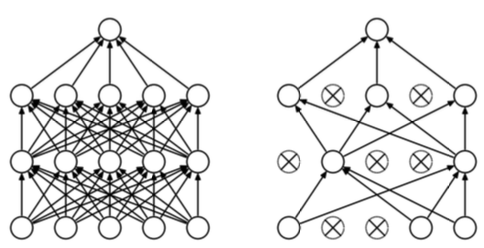
\includegraphics[width=0.7\linewidth]{dropout-net}}
\end{figure}



En un principio parecería que esto perjudica al modelo, pero al eliminar algunos de los pesos el modelo evita centrarse en características individuales de cada ejemplo de clasificación, obligándolo a generalizar más rápido \parencite{dropout}.

Un pequeño experimento en un modelo más avanzado (VGG con \textit{batch normalization} y aumento de datos) permite ver  como afecta el \textit{dropout} a la puntuación final. En la figura \ref{dropout} se puede observar que la mejor puntuación se alcanza eliminando el 45\% de las activaciones, consiguiendo una mejora de un 25\% sobre el modelo que usa todas las activaciones.

\begin{figure}
    \caption{Evolución de la puntuación de un modelo usando \textit{dropout}}
\label{dropout}
  \makebox[\textwidth]{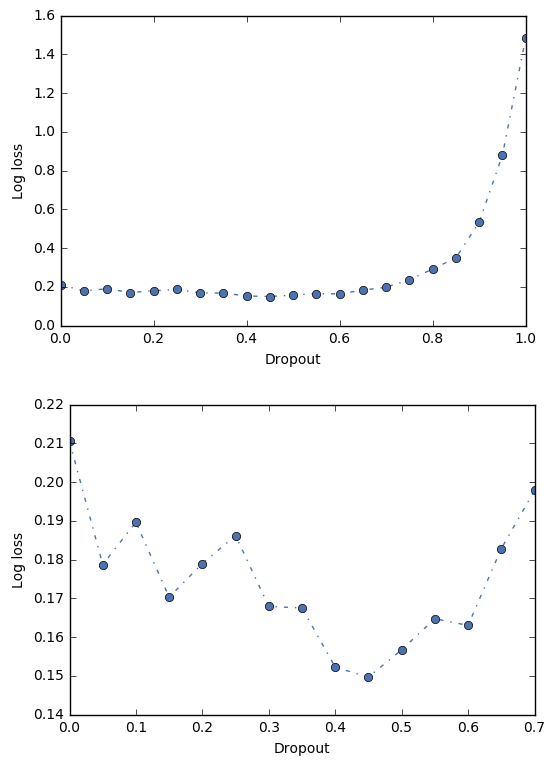
\includegraphics[width=0.7\linewidth]{dropout}}
\end{figure}


También se ve que el modelo empieza a perder eficacia a partir del 70\% de \textit{dropout}, empeorando el modelo original. Esto significa que el modelo es capaz de generalizar con información útil incluso cuando solo posee el 30\% de las activaciones.

Por otra parte también es importante pensar dónde se pierden las activaciones. Por un lado, perder demasiadas activaciones en la entrada sería el equivalente a trabajar sin esos ejemplos. Por otro, perderlos en la salida sería aumentar demasiado el error al clasificar, al no tener tanta capacidad de apoyo en las otras capas.  La idea aplicada aquí es distribuir el \textit{dropout} disminuyéndolo en la entrada y la salida y haciendo que tenga su punto máximo en el centro de la red.

La definición de la red anterior quedaría de la siguiente manera:

\begin{python}
def build_dense_layers(p):
    return [
        Flatten(),
        Dropout(p/4),  # Aplicar 1/4 del dropout definido (p)
        Dense(512, activation='relu'),
        Dropout(p),
        Dense(512, activation='relu'),
        Dropout(p/2),  # Aplicar la mitad del dropout definido
        Dense(8, activation='softmax'),
    ]
dense_model = keras.models.Sequential(build_class_layers(0.45))
\end{python}

Los resultados obtenidos con esta configuracion no mejoran los resultados de la red anterior, pero como se ve en la figura \ref{dropout} sí que lo hará a posteriori, cuando se le apliquen otro tipo de modificaciones al modelo. Modelos como VGG ya incluyen \textit{dropout} (solo en las redes densas), por lo que al hacer fine-tuning con una red personalizada es necesario usarlo para mantener los resultados originales.

\subsection{Normalización por lotes}

En muchos campos del aprendizaje automático es normal normalizar las entradas de los modelos. Normalizar un conjunto de entradas hace que todas estén en la misma escala. Si existe una entrada mucho mayor o menor que el resto esta puede hacer que el entrenamiento arrastre un error mayor del necesario, produciendo inestabilidad y dificultando la convergencia del modelo.

El caso de las redes neuronales no es una excepción. Una entrada con un valor demasiado grande puede llevar a tener un peso determinado demasiado grande para contrarrestarla.

Una normalización estándar en aprendizaje automático es restar de cada entrada el valor medio del conjunto de datos y luego dividirlo por la desviación estándar del mismo. Esto aún presenta problemas para casos como el de este proyecto donde se usa el gradiente del descenso estocástico (cita a su definición en basicos:ann).

Los modelos principales citados en este trabajo: \cite{krizhevsky2012imagenet} y \cite{simonyan} usan sus propias técnicas de normalización, aparte de usar activaciones \textit{ReLu} (cap. \ref{cap:relu}) que son menos sensibles a los datos de entrada sin normalizar. Sin embargo en 2015 se presenta una técnica muy interesante de normalización que cuadra muy bien con el gradiente del descenso estocástico: la normalización por lotes (o \textit{batch normalization}) \parencite{batch_normalization}.

La diferencia con una normalización estándar es que al terminar de normalizar las entradas de una capa se multiplican estas entradas por un parámetro aleatorio, y luego se suma por otro, cambiando así la desviación estándar y la media de la entrada. Estos estos cuatro parámetros (los dos parámetros nuevos, la desviación estándar y la media) se hacen entonces entrenables como pesos del modelo.

Los modelos actualues que usan esta normalización por lotes consiguen la misma precisión que los modelos sin ella usando catorce veces menos pasos de entrenamiento \parencite{batch_normalization}.

Para aplicar esta normalización por lotes al modelo que se está entrenando hay que añadir las capas de normalización por lotes (también disponibles en Keras) al modelo denso:

\begin{python}
def build_dense_layers(p):
    return [
        BatchNormalization(axis=1),
        Flatten(),
        Dropout(p/4),
        Dense(512, activation='relu'),
        BatchNormalization(),
        Dropout(p),
        Dense(512, activation='relu'),
        BatchNormalization(),
        Dropout(p/2),
        Dense(8, activation='softmax'),
    ]
dense_model = keras.models.Sequential(build_class_layers(0.45))
\end{python}

Esto no es suficiente. A diferencia del dropout, la normalización por lotes si que es capaz de mejorar la red convolucional del modelo preentrenado. Gracias a la popularidad de esta técnica y de los modelos preentrenados que se usan en este trabajo ya existen entrenamientos del modelo VGG original usando normalización por lotes, ahorrando la necesidad de entrenar una red tan grande. Una descripción de esto entrenamientos se puede encontrar en \cite{pretrained_with_bn}.

En el caso de este trabajo se ha adaptado bajo la clase $Vgg16BN$. Al cambiar la red convolucional original hay que volver a transformar el conjunto de datos que se usaba para obtener los resultados de aplicar los filtros actualizados sobre las imágenes de entrada.

\begin{python}
# Carga del modelo VGG16 con normalizacion por lotes
from vgg16bn import Vgg16BN
import utils
model = Vgg16BN()
conv_model, _ = utils.split_at(model, MaxPooling2D)

# Cargamos los diferentes conjuntos de datos
train, trail_labels = get_data(path + 'train')
valid, valid_labels = get_data(path + 'valid')
test, test_labels = get_data(path + 'test')

# Convertir dataset a features mediante la red convolucional 
train_feat = conv_model.predict(train)
valid_feat = conv_model.predict(valid)
test_feat = conv_model.predict(test)

# Entrenar la red
dense_model = keras.models.Sequential(build_class_layers(0.45))
dense_model.compile(...)
dense_model.fit(...)
# Evaluar el modelo sobre el conjunto de test
dense_model.evaluate(test_feat, test_labels)
>>> [0.16719577019912478, 0.9611234577100389]
\end{python}

Como se puede apreciar, los dos últimos cambios han supuesto una mejora considerable sobre el modelo anterior, clasificando correctamente el 96\% de los ejemplos del conjunto de test.

TODO: poner aqui la clasificacion de kaggle de este modelo, que es uno de los presentados.


\subsection{Aumento de datos}

Una de los principales obstáculos de este problema es el reducido tamaño del conjunto de datos de entrenamiento. El tener pocos ejemplos sobre los que entrenar hace que al modelo le cueste generalizar sobre los ejemplos dispoibles, generando un sobreajuste del problema.

Otro de los métodos para reducir el sobreajuste del modelo es llamado aumento de datos (\textit{data augmentation}). Se trata de generar más imágenes de entrenamiento usando las ya disponibles, rotando la imagen original, aumentándola, cambiando ligeramente el color, etc. 

En el caso de este problema es especialmente interesante, ya que las cámaras de los barcos están fijas apuntando siempre a la misma zona. Al hacer fotos sobre los peces capturados, siempre suelen estar con la cabeza apuntando en dirección contraria al agua. Esto podría hacer que la red encuentre fácil reconocer peces apuntando en una dirección pero difícil en otra. Si las redes convolucionales ayudaban a detectar determinados patrones en cualquier punto de la imagen, el aumento de datos ayudará a liberarnos de otras variantes como la rotaciónm, el tamaño o el filtro de color dado por el ambiente.

Un ejemplo se puede observar en la imagen de la figura \ref{aug-original}, con algunas de las transformaciones aplicadas vistas en la figura \ref{augmentations}.

\begin{figure}
    \caption{Imagen del conjunto de datos}
\label{aug-original}
  \makebox[\textwidth]{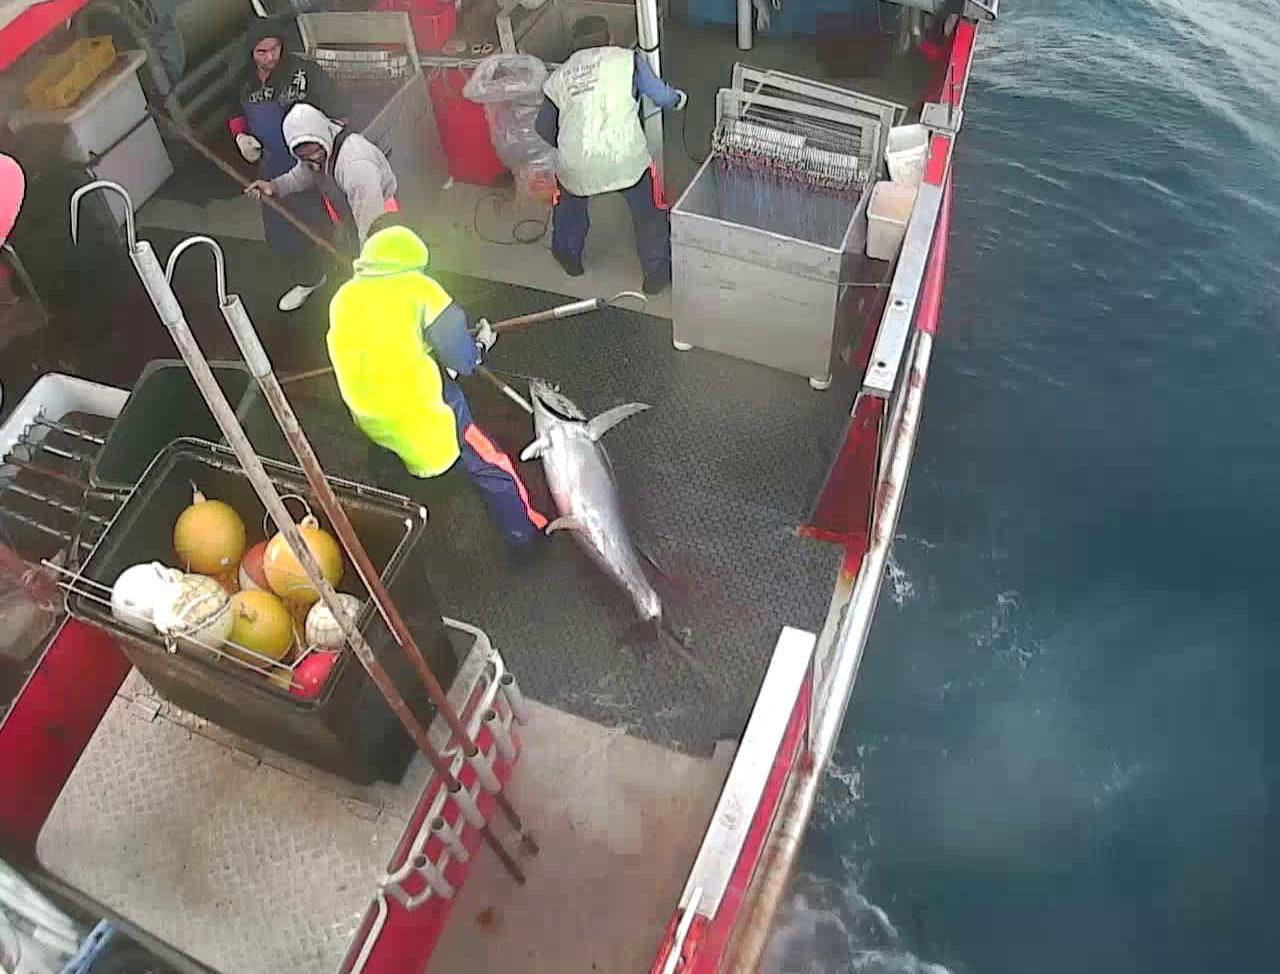
\includegraphics[width=0.7\linewidth]{aug-original}}
\end{figure}

\begin{figure}
    \caption{Cuatro aumentos diferentes de la imagen, reescalada a $224\times224$ píxeles}
\label{augmentations}
  \makebox[\textwidth]{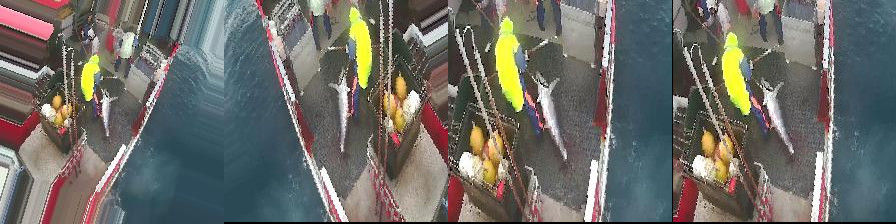
\includegraphics[width=\linewidth]{augmentations}}
\end{figure}

Para generar aumentos de datos en Keras hay que mirar la clase que hasta ahora se había usado para importar el conjunto de datos. Keras está estructurado para trabajar con grandes conjuntos de datos, por lo que ha implementado un generador de imágenes a partir de un directorio de imágenes. Se puede aprovechar las opciones de este generador para construir nuevas imágenes usando diferentes transformaciones.

En este caso se usaba la utilidad $gen\_data()$, que encapsulaba la llamada al generador de datos. Ahora se definirá una nueva función que usa un generador de imágenes personalizado.

Si es neccesario saber como se aplican las transformaciones a las diferentes imágenes es posible especificar un directorio de salida al generador de imágenes para que las vaya guardando en dicho directorio.

\begin{python}
# Crear el generador de imagenes
image_generator = image.ImageDataGenerator(
    rotation_range=30,
    horizontal_flip=True,
    zoom_range=0.4,
)

batches = img_gen.flow_from_directory(
    path+'test_aug', 
    target_size=(224,224),
    class_mode='categorical',
    shuffle=False,
    batch_size=4,
    save_to_dir=path+'augmentation',
)

# Iterar sobre batches para extraer los datos
# En este caso se sacan 4 veces la cantidad de datos originales
data = [batch.next() for _ in range(batches.nb_samples * 4)]
\end{python}

Ahora no es necesario modificar el modelo, solo reentrenarlo con los nuevos datos. Como ha ocurrido antes, al cambiar el conjunto de datos hay que transformarlo pasándolo por la red convolucional, usando en este caso la última versión con normalización por lotes.

Lo interesante de ver en este caso es como se ha reducido el sobreajuste durante el entrenamiento.

\begin{python}
Epoch 5/7
loss: 0.0768 - acc: 0.9817 - val_loss: 0.1142 - val_acc: 0.9538
Epoch 6/7
loss: 0.0639 - acc: 0.9895 - val_loss: 0.1212 - val_acc: 0.9334
Epoch 7/7
loss: 0.0708 - acc: 0.9860 - val_loss: 0.1139 - val_acc: 0.9520

dense_model.evaluate(test_feat, test_labels)
>>> [0.15222558558899649, 0.96723868954758185]
\end{python}

El modelo, que ahora ha predecido casi un 97\% de las imágenes del conjunto de test ha aumentado ligeramente la puntuación de pérdida logarítmica. Hay que tener en cuenta que a medida que la puntuación se va acercando a cero es más difícil disminuir la puntuación, ya que se está acercando a un modelo casi perfecto. 

Cuando se habla de un modelo casi perfecto se habla refiriéndose al conjunto de test elegido. En este caso, debido al pequeño tamaño del conjunto de test, la perfección del modelo estará lejos de la perfección del modelo real que va a ser probado en el concurso.


\section{Modelo convolucional}

Hasta ahora se ha seguido siempre la misma estructura: una vez transformado el conjunto de datos se entrenaba un red densa (completamente conectada) de tres capas. Una parte del preprocesamiento de las imágenes era redimensionarlas a un tamaño más manejable, de $224\times224$.

Una de las ventajas de las redes convolucionales es que permite aumentar el tamaño de las imágenes elegidas sin aumentar la complejidad de la red, ya que el número de pesos no cambiaría, solo el tamaño de la salida. Sin embargo, al tener una red neuronal estándar a la salida de la red convolucional esta si que aumentaría muchísimo con el cambio de tamaño de las imágenes.

Para intentar aprovechar esta facilidad que ofrecen las redes convolucionales se puede hacer una clasificación directamente usando redes convolucionales en todo el proceso, clasificando al final con única capa de activación clásica.

Aquí se estaría desarrollando una idea que se comentaba al principio de este trabajo, el conseguir ocho filtros cuya salida sea la probabilidad que en la zona de la imagen esté apareciendo el pez de la clase elegida.

\begin{python}
def build_conv_layers():
    return [
        BatchNormalization(axis=1, 
            input_shape=conv_layers[-1].output_shape[1:]
        ),
        Convolution2D(128, 3, 3, activation='relu', border_mode='same'),
        BatchNormalization(axis=1),
        Convolution2D(128, 3, 3, activation='relu', border_mode='same'),
        BatchNormalization(axis=1),
        Convolution2D(128, 3, 3, activation='relu', border_mode='same'),
        BatchNormalization(axis=1),
        Convolution2D(8, 3, 3, border_mode='same'),
        
        # Output layer
        GlobalAveragePooling2D(),
        Activation('softmax'),
    ]
\end{python}

La idea es usar tres capas de convoluciones, con 128 filtros cada una. La combinación de estos 128 filtros permitirá capturar la combinatoria de caracterísicas que representa la red convolucional preentrenada. Al final se añade una última capa de convolución, cada una representando los filtros de cada clase.

Las imágenes resultantes de estos filtros se transforman a una sola entrada usando una capa \textit{GlobalAveragePooling2D}. Esta capa funciona como las capas POOL de la red convolucional, pero usando el toma la imagen en vez de la cercanía de cada uno de los píxeles, generando una salida que pueda ser entendida por la capa de activación.

De nuevo habrá que transformar el conjunto de datos pasándolo por la red convolucional preentrenada, ya que se va a usar un tamaño de imagen de $360\times640$.

Aunque, como se ha comentado, la red convolucional acepta un aumento del tamaño de la imagen sin aumentar exponencialmente los tiempo de entrenamiento, el entrenar una red convolucional es mucho más costoso que una red clásica. Esto se debe a que hay que actualizar $n\timesn$ pesos por cada píxel de cada imagen. En este caso el entrenamiento de la red completamente convolucional ha tardado 24 veces más que el entrenamiento de la red densa del capítulo anterior.

\begin{python}
conv_model.evaluate(test_feat, test_labels)
>>> [0.14251796898005481, 0.973238231345685]
\end{python}

Al evaluar el modelo se ve que consigue una pequeña mejora respecto al modelo denso. Pero el aumento de puntuación no es la única ventaja de este modelo.

\subsection{Visualización del modelo}

El hecho de que en ningún momento hasta la clasificación se haya dejado de trabajar con redes convolucionales hace que siempre se haya trabajo con filtros aplicado a imágenes. Como se decía antes, la idea abstracta era conseguir filtros que resaltaran la posibilidad de la existencia de un pez de esa clase en cada zona de la imagen.

Se puede usar los diferentes pesos de los filtros para construir un mapa de calor sobre el filtro de clasificación de su clase. Si se redimensiona el filtro (ya que ha sido reducido por las capas de MaxPooling2D) al tamaño de la imagen original se puede ver como encuentra el pez a clasificar en cada imagen. Un ejemplo de esto se puede ver en la figura \ref{fc-heatmap}.

\begin{figure}
    \caption{Una imagen correspondiente a la clase ALB: \textit{Thunnus alalunga}}
\label{fc-fish}
  \makebox[\textwidth]{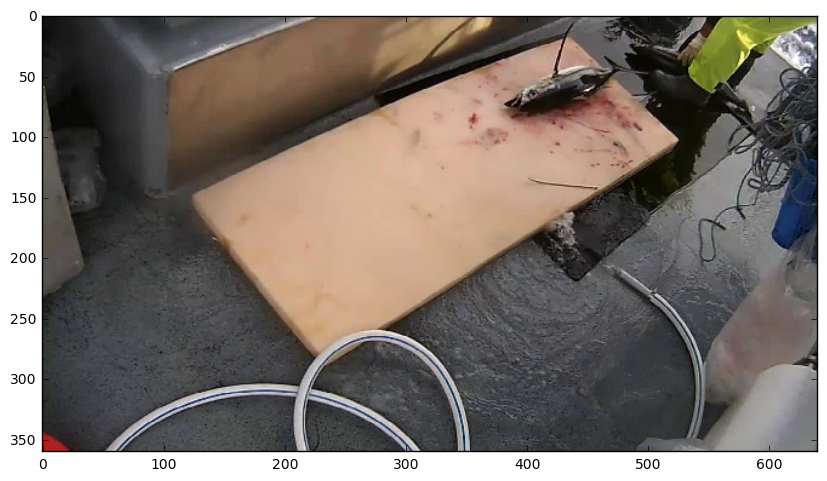
\includegraphics[width=\linewidth]{fc-fish}}
\end{figure}

\begin{figure}
    \caption{Aplicación del mapa de calor reescalado a la imagen \ref{fc-fish}}
\label{fc-heatmap}
  \makebox[\textwidth]{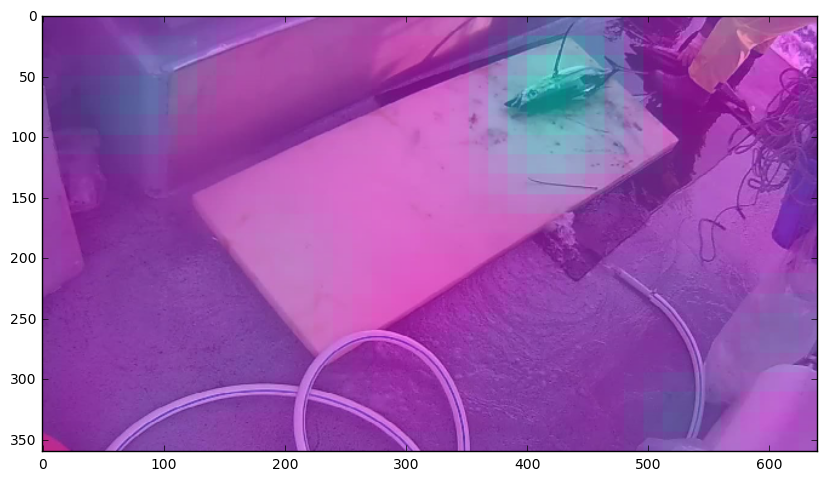
\includegraphics[width=\linewidth]{fc-heatmap}}
\end{figure}

Esto no solo permite comprobar que el modelo funciona correctamente, sino buscar los ejemplos que peor clasifica y comprobar que está señalando el mapa de calor correspondiente.

Un ejemplo claro de como se puede usar esta técnica de visualización para detectar los errores en el modelo es cuando se intenta clasificar un atún de cola amarilla (YFT: \textit{Thunnus albacares}), en la imagen \ref{yft}.

Una característica de los atunes de cola amarilla es su banda de tonos amarillos en el lomo, característica que el modelo podría haber aprendido gracias a los ejemplos. Sin embargo la imagen \ref{yft} muestra el atún visto desde abajo, con las aletas abiertas. Esto deja una de las características del atún escondida, siendo difícil clasificarlo incluso para un humano no familiarizado con atunes.

Al mostrar el mapa de calor del YFT en la imagen \ref{yft-heatmap} se puede apreciar que la hipótesis de que el modelo ha aprendido a detectar los atunes de cola amarilla a través del color podría ser cierta, ya que una de las partes más importantes de la foto para el filtro son los pantalones del pescador, de un color amarillo fuerte.

Esto pertime tomar ciertas decisiones sobre el entrenamiento del modelo. Por ejemplo, si se ve que la fijación del modelo con el color es un error y es preferible que use otras cosas como formas o texturas se puede eliminar el color de las imágenes o aumentar los datos usando transformaciones de color que hagan especial hincapié en la varianza del color amarillo.

\begin{figure}
    \caption{Una imagen correspondiente a la clase ALB: \textit{Thunnus alalunga}}
\label{yft}
  \makebox[\textwidth]{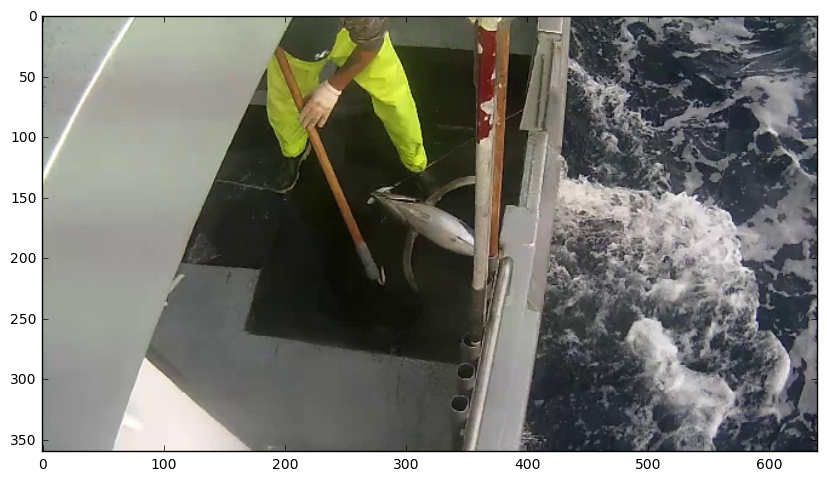
\includegraphics[width=\linewidth]{yft}}
\end{figure}

\begin{figure}
    \caption{Aplicación del mapa de calor reescalado a la imagen \ref{fc-fish}}
\label{yft-heatmap}
  \makebox[\textwidth]{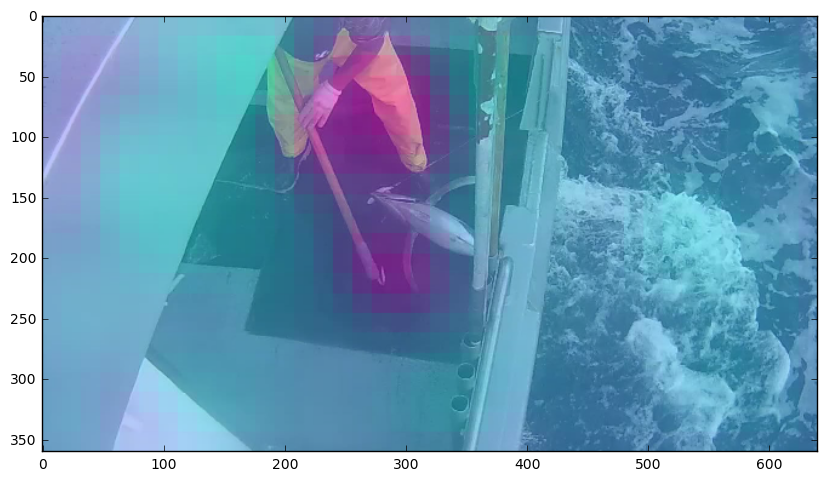
\includegraphics[width=\linewidth]{yft-heatmap}}
\end{figure}

\section{Modelo con entrada múltiple}

Una examinación del conjunto de datos de entrada nos permite averiguar determinadas propiedades de las imágenes que se podrían usar para una mejora de los modelos. Por ejemplo, las imágenes están sacadas de diferentes barcos, con diferentes modelos de cámaras. No todas las cámaras generan imágenes del mismo tamaño, por lo que se puede averiguar el barco del que se ha tomado la fotografía por el tamaño de la imagen. 

Ya que diferentes barcos suelen pescar diferentes tipos de peces con mayor o menor probabilidad, el conseguir el tipo de barco puede ser aprovechado por el modelo para balancear las posibilidades de una clase dependiendo del tipo de pesca que suela llevar.

Obviamente la idea no es hacer todo esto a mano, si no entrenar un modelo que tenga en cuenta tanto las imágenes como otra información válida. En este caso se va a elegir el modelo denso, con la diferencia que la última capa tendrá dos entradas: la salida de las capas ocultas de la red neuronal y el tamaño de la imagen, codificado en \textit{onehot}.

TODO Hacer un esquema de las arquitectura de la red.

\begin{python}
def build_dense_layers(p):
    # Usamos las entradas de la red convolucional, como antes
    inp = Input(conv_layers[-1].output_shape[1:])
    x = MaxPooling2D()(inp)
    x = BatchNormalization(axis=1)
    x = Flatten()
    x = Dropout(p/4)
    x = Dense(512, activation='relu')
    x = BatchNormalization()
    x = Dropout(p)
    x = Dense(512, activation='relu')
    x = BatchNormalization()
    x = Dropout(p/2)

    # Aqui usamos las entradas de los tamaños de las imágenes
    size_inputs = Input(len(sizes))
    bn_inputs = BatchNormalization()(size_inputs)

    # Mergeamos ambas entradas en una última capa
    x = merge([x, bn_inp], 'concat']
    x = Dense(8, activation='softmax')
    return x

dense_model = keras.models.Model(
    [inp, size_inputs],  # El modelo ahora tiene multi entrada
    build_class_layers(0.45)
)
\end{python}

Tras construir el modelo con las entradas múltiples y entrenarlo sobre los dos conjuntos de entrenamiento (las imágenes y los tamaños de las imágenes) vemos la evaluación del modelo.
\begin{python}
dense_model.evaluate(test_feat, test_labels)
>>> [0.1725, 0.9413]
\end{python}

El modelo ha sacado una evaluación peor que modelos anteriores, incluso usando un modelo que ya se conocía con una evaluación superior.

Aunque la idea es buena, lo que está haciendo por debajo es clasificar los diferentes barcos en base a los tamaños de sus imágenes. Debido a la amplia diferencia de las imágenes de los diferentes tipos de barcos, ya sea por los colores, iluminación, objetos, etc, el modelo denso probablemente ya esté teniendo en cuenta de qué barco es cada imagen. Por lo tanto lo único que va a añadir el introducir estos datos es complejidad del modelo, haciendo más difícil converger a un modelo bueno.

\subsubsection{Fuga de datos}

Esta idea de usar datos diferentes del dataset para clasificar es algo muy usado en los torneos de modelos predictivos. No solo funciona el tamaño de la foto, sino a veces las fotos tienen datos adicionales, como información GPS, hora de creación o modelo de cámara.

No todos estos datos son publicados de una manera voluntaria por comunidades de campeonatos, pero son útiles para conseguir una pequeña mejora en el modelo, siempre que el modelo puede aprovecharse de estos datos.

\section{Salida múltiple}

Se ha explorado la idea de usar un modelo que tenga diferentes fuentes de entrada. También se puede intentar un modelo con diferentes salidas. Una idea no solo es averiguar qué tipo de pez es sino también donde se encuentra en la foto.

Esta estructura hará que el modelo tenga que predecir dos cosas al mismo tiempo, lo cual hace que sea más difícil una convergencia de este. Por otro lado si consige una buena puntuación tiene menos probabilidades de fallar. Si se mira el ejemplo de los pantalones amarillos de la red completamente convolucional, debería encontrar el pez en la foto y a la vez clasificar la foto. En la foto era capaz de predecir que el pez era un atún de cola amarilla por las razones incorrectas, pero en este caso no será capaz ya que tendrá la localización incorrecta del pez.

Para entrenar las localizaciones de los peces en las imágenes se ha usado el dataset que uno de los usarios de kaggle ha hecho público: un conjunto con las coordenadas rectángulos que contienen un pez en la imagen ).
\begin{figure}
  \caption{Ejemplo del dataset de localizaciones de peces}
\label{box}
  \makebox[\textwidth]{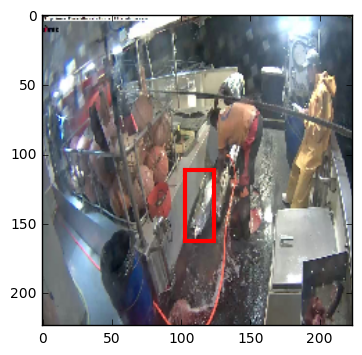
\includegraphics[width=0.5\linewidth]{box}}
\end{figure}

